\section{Design}
\label{s:gen}

\autoref{f:flow} shows \sys's workflow.  Based on the LLVM intermediate
representation~(IR) compiled from source code, \sys generates a set
of constraints for each integer operation, and feed them into the
constraint solver.

Particularly, \sys generates three types of constraints.
%
Given an integer operation, \sys generates its error constraint
directly from the definition.
%
\sys also calculates the path constraint, the predicate satisfying
which the operation is reachable from the start of that function.
%
To further improve accuracy, \sys infers additional integral ranges
of function parameters and structure fields across the call graph,
and also allows users to provide range annotations.

\begin{figure}
\centering
\resizebox{0.9\linewidth}{!}{
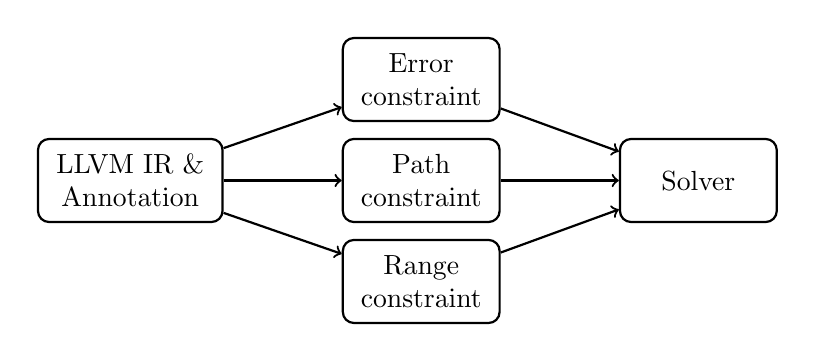
\begin{tikzpicture}[
	block/.style={
		rectangle, rounded corners,
		draw=black, thick,
		text width=5em, minimum height=3em, text centered
	},
	line/.style={draw, thick, ->},
	]
	\matrix[row sep=2mm, column sep=15mm] {
		& \node [block] (ec) {Error constraint}; & \\
		\node [block, text width=6em] (ir) {LLVM IR \& Annotation};
		& \node [block] (pc) {Path constraint};
		& \node [block] (sol) {Solver}; \\
		& \node [block] (rc) {Range constraint}; & \\
	};

	\path [line] (ir) -- (ec);
	\path [line] (ir) -- (pc);
	\path [line] (ir) -- (rc);
	\path [line] (ec) -- (sol);
	\path [line] (pc) -- (sol);
	\path [line] (rc) -- (sol);
\end{tikzpicture}

}
\caption{\sys's workflow.  It generates constraints from the LLVM
intermediate representation~(IR) and user annotations, and then feeds
the constraints to a solver for satisfiability testing.}
\label{f:flow}
\end{figure}

\subsection{Error Constraint Generation}

One may implement the error constraints defined in \autoref{s:sema:constr}
as Boolean circuits for deciding satisfiability.  For example, given
two $n$-bit unsigned integers, the multiplication error constraint
could be implemented using a $2n$-bit binary multiplier, which flags
an overflow error if any of the most significant $n$ bits of the
product is 1.

The Boolector constraint solver provides several highly optimized
circuits to implement these error constraints.  As for the
multiplication error constraint, Boolector's overflow detection
circuit does not even need to compute the $2n$-bit product first
and can be solved more
efficiently~\cite[\chapterautorefname~3.5]{brummayer:phd}.  \sys
reuses them to generate error constraints for better performance.

\subsection{Path Constraint Generation}

use \autoref{f:ax25-sign} as an example.

unroll loops once.

Move in-loop constraints out.

handle comparison like \cc{p == NULL}.

\begin{figure}
\begin{algorithmic}
\Function{PathConstraint}{$\mathit{blk}$}
\State $g \gets \textbf{false}$
\ForAll{$\mathit{pred} \in \mathit{blk}$'s predecessors(s)}
\State $e \gets (\mathit{pred},\mathit{blk})$
\If{$e$ is not a back edge}
	\State $\mathit{br} \gets e$'s branching condition
	\State $\mathit{as} \gets \bigwedge_i(x_i = y_i)$ for all assignments along $e$
	\State $g \gets g \lor (\Call{PathConstraint}{\mathit{pred}} \land \mathit{br} \land \mathit{as})$
\EndIf
\EndFor
\State \Return{$g$}
\EndFunction
\end{algorithmic}

\caption{Algorithm for path constraint generation.}
\label{f:path-cstr}
\end{figure}

\subsection{Range Constraint Generation}

Range constraint \& annotations?

handle sysctl interface.


\subsection{Optimization}

false error \& performance.

\paragraph{Pointer arithmetic.}
\sys represents each pointer or memory address as a symbolic
expression~\cite{engelen:symbolic}, and tries to simplify it if
possible.  A pointer expression that \sys fails to simplify will
be considered as a black-box integer, which can be any value within
its range.  Consider the code snippet below.
%
\begin{Verbatim}[commandchars=\\\{\},codes={\catcode`\$=3\catcode`\^=7\catcode`\_=8}]
\PY{k}{struct} \PY{n}{pid\PYZus{}namespace} \PY{p}{\PYZob{}}
    \PY{k+kt}{int} \PY{n}{kref}\PY{p}{;}
    \PY{k}{struct} \PY{n}{pidmap} \PY{n}{pidmap}\PY{p}{[}\PY{n}{PIDMAP\PYZus{}ENTRIES}\PY{p}{]}\PY{p}{;}
    \PY{p}{.}\PY{p}{.}\PY{p}{.}
\PY{p}{\PYZcb{}}\PY{p}{;}
\PY{k}{struct} \PY{n}{pid\PYZus{}namespace} \PY{o}{*}\PY{n}{pid\PYZus{}ns} \PY{o}{=} \PY{p}{.}\PY{p}{.}\PY{p}{.}\PY{p}{;}
\PY{k+kt}{unsigned} \PY{k+kt}{int} \PY{n}{last} \PY{o}{=} \PY{p}{.}\PY{p}{.}\PY{p}{.}\PY{p}{;}
\PY{k}{struct} \PY{n}{pidmap} \PY{o}{*}\PY{n}{map} \PY{o}{=}
    \PY{o}{&}\PY{n}{pid\PYZus{}ns}\PY{o}{-}\PY{o}{>}\PY{n}{pidmap}\PY{p}{[}\PY{p}{(}\PY{n}{last} \PY{o}{+} \PY{l+m+mi}{1}\PY{p}{)}\PY{o}{/}\PY{n}{BITS\PYZus{}PER\PYZus{}PAGE}\PY{p}{]}\PY{p}{;}
\PY{k+kt}{int} \PY{n}{off} \PY{o}{=} \PY{n}{map} \PY{o}{-} \PY{n}{pid\PYZus{}ns}\PY{o}{-}\PY{o}{>}\PY{n}{pidmap}\PY{p}{;}
\end{Verbatim}

%
The offset of \cc{pidmap} in the structure \cc{pid_namespace} is 4
bytes, i.e., the size of \cc{kref}, thus \sys represents the address
\cc{pid_ns->pidmap} as $\cc{pid_ns} + 4$.  Here \cc{pid_ns} is
considered as a black box since no further information is available.

In addition, assuming the size of each element of \cc{pidmap} is 8
bytes, \sys represents the address \cc{\&pid_ns->pidmap[i]} as
$\cc{pid_ns} + 4 + i \times 8$; in this example we have $i =
(\cc{last} + 1) /_u \cc{BITS_PER_PAGE}$.  Thus, the value of \cc{off},
the subtraction of the two pointers, is reduced to $(\cc{pid_ns} +
4 + i \times 8) - (\cc{pid_ns} + 4) = i \times 8$.

\paragraph{Value equality testing.}
How to determine the values from two load instructions
are the same? Load hoisting, unsound aliasing rules.

\autoref{f:hoist} shows in the hoisting algorithm.

aliasing assumption~\cite{livshits:ipssa}.
\sys assumes that a pointer passed as a function parameter or a
global variable points is distinct from any other memory location.


\begin{figure}
\begin{algorithmic}
\footnotesize
\Procedure{Hoist}{$I$}\Comment{$I$ is a load instruction}
\State $\mathit{loc} \gets I$'s memory location to load from
\Loop
\If{\textbf{not} \Call{HoistInBlock}{$I$, $\mathit{loc}$}}
	\State \Return
\EndIf
\State $\mathit{blk} \gets$ \Call{ChooseTargetBlock}{$I$, $\mathit{loc}$}
\If{$\mathit{blk} = \textbf{nil}$}
	\State \Return
\EndIf
\State Move $I$ to the end of $blk$
\EndLoop
\EndProcedure
\\
\Function{HoistInBlock}{$I$, $\mathit{loc}$}
\Loop
\State $\mathit{prev} \gets I$'s previous instruction in current block
\If{$\mathit{prev} = \textbf{nil}$}
	\Comment{Moved to beginning of the block?}
	\State \Return \textbf{true}
\EndIf
\If{$\mathit{prev}$ may modify $\mathit{loc}$ \textbf{or} \\
\hspace{3.6em} \textbf{not} $\mathit{loc}$ dominates $\mathit{prev}$}
	\State \Return \textbf{false}
\EndIf
\State Move $I$ before $\mathit{prev}$
\EndLoop
\EndFunction
\\
\Function{ChooseTargetBlock}{$I$, $\mathit{loc}$}
\State $\mathit{blk} \gets I$'s block
\State $\mathit{anc} \gets$ the common ancestor of $\mathit{blk}$'s predecessor(s)
\If{$\mathit{anc} = \mathit{blk}$ \textbf{or} \textbf{not} $\mathit{loc}$ dominates $\mathit{anc}$}
	\State \Return \textbf{nil}
\EndIf
\State $\mathit{blkset} \gets \{\mathit{anc}\}$
\If{\Call{CanBlocksModify}{$\mathit{loc}$, $blk$, $\mathit{blkset}$}}
	\State \Return \textbf{nil}
\EndIf
\State \Return $\mathit{anc}$
\EndFunction
\\
\Function{CanBlocksModify}{$\mathit{loc}$, $\mathit{blk}$, $\mathit{blkset}$}
\ForAll{$b \in \mathit{blk}$'s predecessor(s)}
	\If{$b \notin \mathit{blkset}$}
		\State $\mathit{blkset} \gets \mathit{blkset} \cup \{b\}$
		\ForAll{$\mathit{instr} \in b$}
			\Comment{Can $b$ modify $\mathit{loc}$?}
			\If{$\mathit{instr}$ may modify $\mathit{loc}$}
				\State \Return \textbf{true}
			\EndIf
		\EndFor
		\If{\Call{CanBlocksModify}{$\mathit{loc}$, $b$, $\mathit{blkset}$}}
			\State \Return \textbf{true}
		\EndIf
	\EndIf
\EndFor
\State \Return \textbf{false}
\EndFunction

\end{algorithmic}

\caption{The hoisting algorithm to move a load instruction to the
earliest possible point within a function.  It repeats the two
phases: first try to move the instruction to the beginning of its
basic block; if successful, try to move it into the common ancestor
of the block's predecessors.}
\label{f:hoist}
\end{figure}

\paragraph{Error-before-check.}
An integer error check may come after the overflowed computation,
but before any use of the result.  In that case, the overflowed
computation is benign.  Below is such an example.  Even the
multiplication $x \times_u y$ overflows, the product \cc{size} is
not used before the check.
\begin{Verbatim}[commandchars=\\\{\},codes={\catcode`\$=3\catcode`\^=7\catcode`\_=8}]
\PY{k+kt}{unsigned} \PY{n}{size} \PY{o}{=} \PY{n}{x} \PY{o}{*} \PY{n}{y}\PY{p}{;}
\PY{k}{if} \PY{p}{(}\PY{n}{x} \PY{o}{\PYZgt{}} \PY{n}{UINT\PYZus{}MAX} \PY{o}{/} \PY{n}{y}\PY{p}{)}
    \PY{k}{return} \PY{o}{-}\PY{l+m+mi}{1}\PY{p}{;}
\PY{p}{.}\PY{p}{.}\PY{p}{.} \PY{o}{=} \PY{n}{malloc}\PY{p}{(}\PY{n}{size}\PY{p}{)}\PY{p}{;}
\end{Verbatim}


To avoid warning against such cases, \sys invokes LLVM to push every
integer operation down to the latest possible point along the control
flow, so that the result is computed only when it is needed.  The
detail of the algorithm is omitted since it is similar to load
hoisting, except that it runs towards the opposite direction, and
does not need to consider memory loads and stores.

In the above example, \sys will move the integer operation $x
\times_u y$ down to right after the \cc{if} branch and before the
\cc{malloc} call, where its result \cc{size} is first used.

\paragraph{Overflowed checking idiom.}

\sys recognizes XXX integer error checking idioms...

\subsection{Limitations}

miss bugs in some configurations, architectures,
and assembly code.
